
We wanted to keep the preprocessing part of our algorithm simple as we found the other stages of the human face authentication pipeline more interesting. In hindsight though we recognize that this phase becomes the foundation determining the amount of work as well as the performance of the other phases. Therefore we should perhaps have put more effort into implementing an algorithm that works better for various lightning conditions and that also normalizes the colors better. An improved version could for example have led to that the proposed algorithm would have been able to correctly detect the face seen in Figure \ref{fig:fail2}. 



% The goal we had in mind for was to implement a face detection algorithm based on the actual color of the images instead of focusing on 

% We are well aware of that our algorithm might seem overly complicated. 

% Ta upp dynamic thresholds etc etc...

% Ta upp disk kernel

% Eigenfaces.

% The face detection part of the algorithm can for example be improved by utilizing the facial expression normalization methods explored in  \cite{facialExpressions}.


\begin{figure}[H]
\centering

\begin{subfigure}{.25\textwidth}
  \centering
  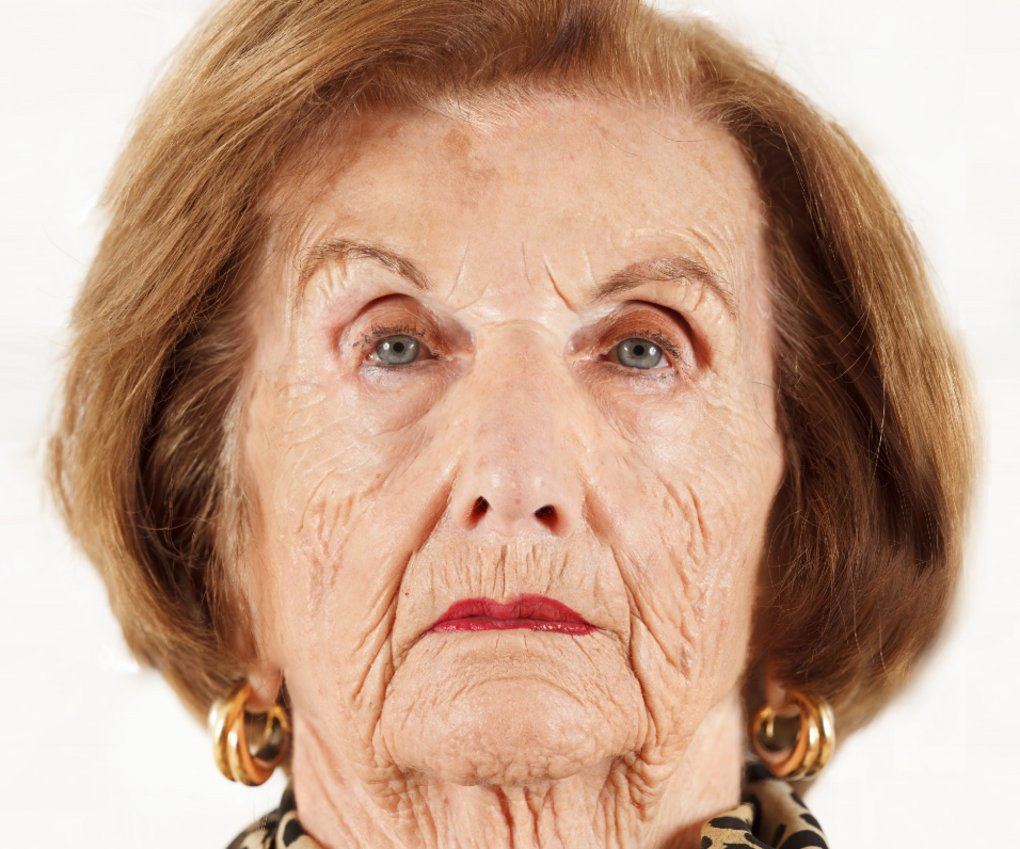
\includegraphics[width=0.95\textwidth]{img/fd3/fail1_input.jpg}
  \caption{}
\end{subfigure}%
\begin{subfigure}{.25\textwidth}
  \centering
  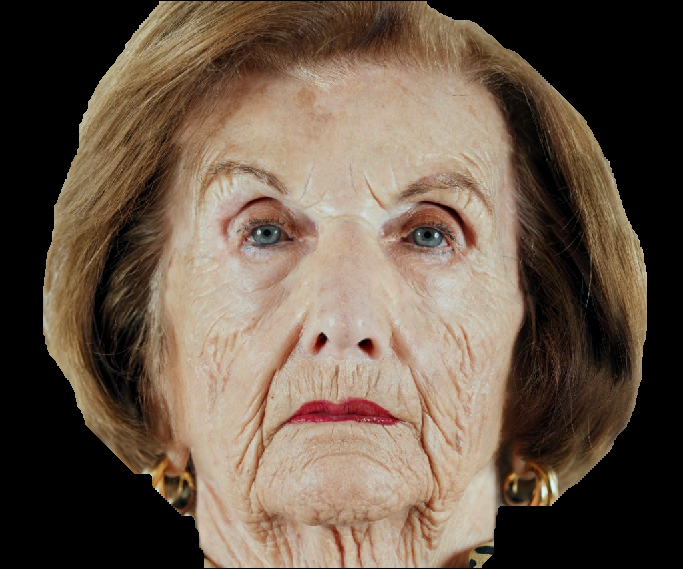
\includegraphics[width=0.95\textwidth]{img/fd3/fail1_faceImage.png}
  \caption{}
\end{subfigure}%
\begin{subfigure}{.25\textwidth}
  \centering
  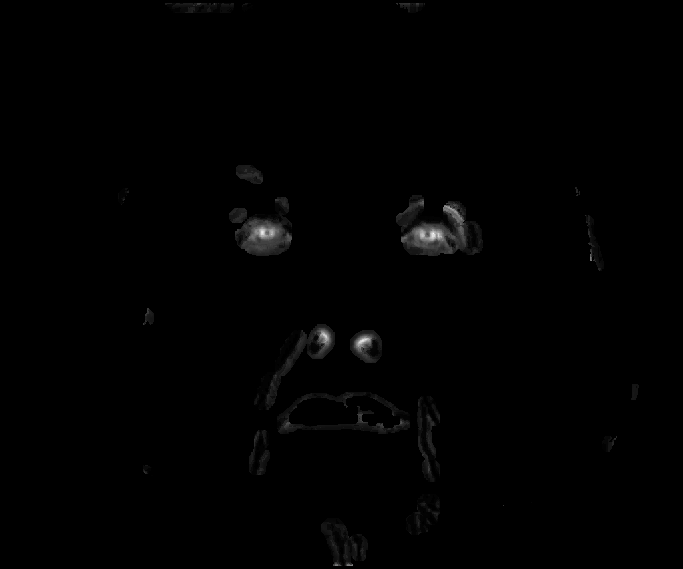
\includegraphics[width=0.95\textwidth]{img/fd3/fail1_finalEyeMap.png}
  \caption{}
\end{subfigure}%
\begin{subfigure}{.25\textwidth}
  \centering
  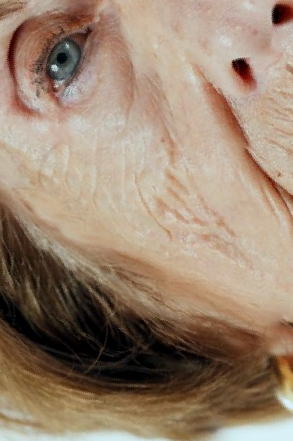
\includegraphics[width=0.53\textwidth]{img/fd3/fail1_output.png}
  \caption{}
\end{subfigure}%

\caption{Resonera, Fail1}
\label{fig:fail1}
\end{figure}


\begin{figure}[H]
\centering

\begin{subfigure}{.25\textwidth}
  \centering
  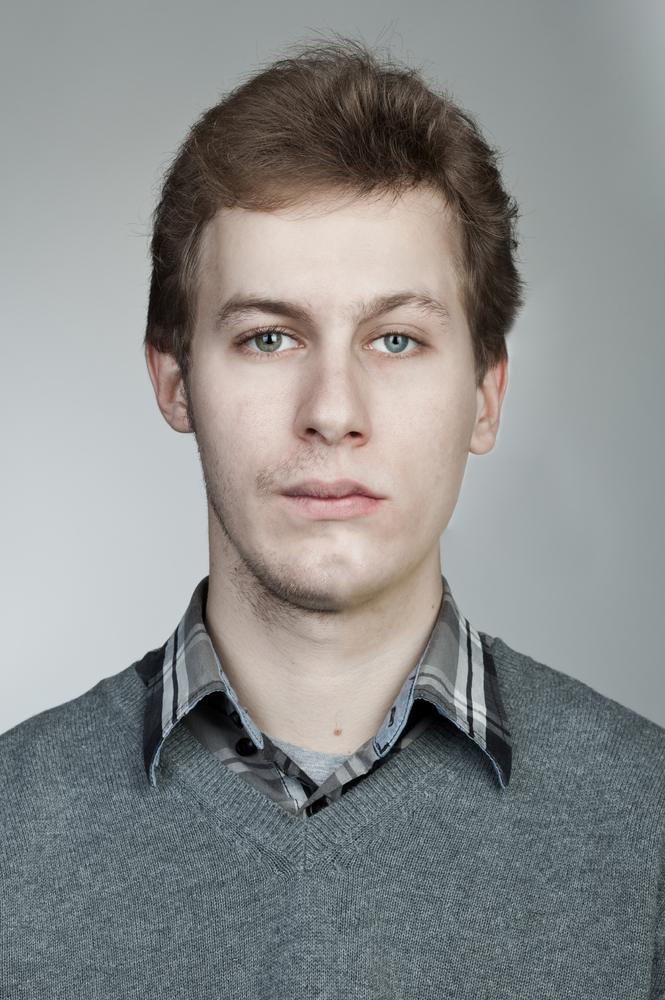
\includegraphics[width=0.53\textwidth]{img/fd3/fail2_input.jpg}
  \caption{}
\end{subfigure}%
\begin{subfigure}{.25\textwidth}
  \centering
  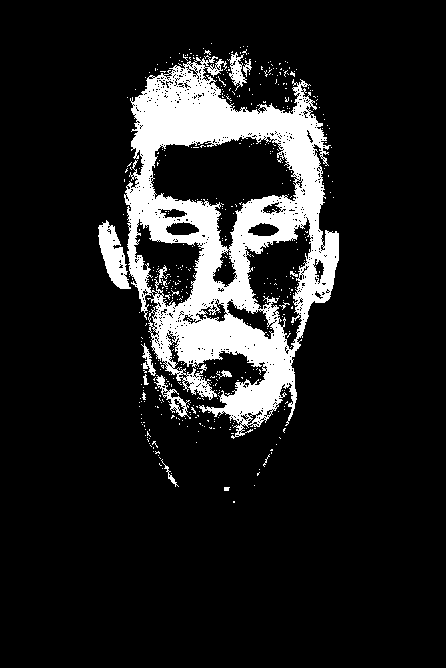
\includegraphics[width=0.53\textwidth]{img/fd3/fail2_estimatedSkinMak.png}
  \caption{}
\end{subfigure}%
\begin{subfigure}{.25\textwidth}
  \centering
  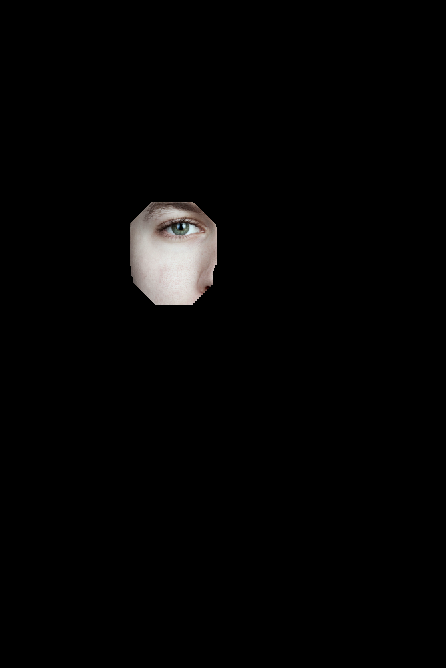
\includegraphics[width=0.53\textwidth]{img/fd3/fail2_faceImage.png}
  \caption{}
\end{subfigure}%
\begin{subfigure}{.25\textwidth}
  \centering
  
\includegraphics[width=0.23\textwidth]{img/fd3/fail2_output.png}
  \caption{}
\end{subfigure}%

\caption{Resonera, Fail2}
\label{fig:fail2}
\end{figure}




\begin{figure}[H]
\centering

\begin{subfigure}{.25\textwidth}
  \centering
  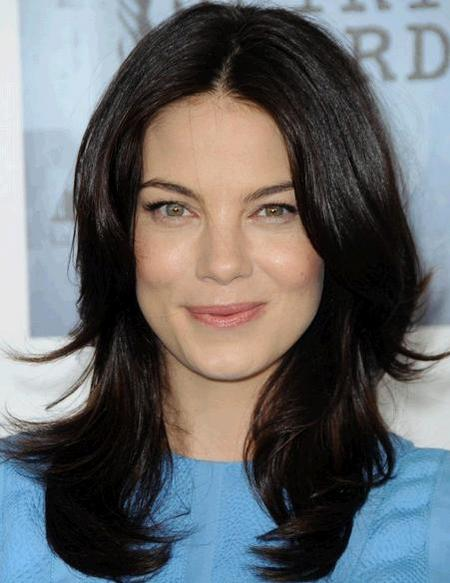
\includegraphics[width=0.53\textwidth]{img/fd3/fail3_input.jpg}
  \caption{}
\end{subfigure}%
\begin{subfigure}{.25\textwidth}
  \centering
  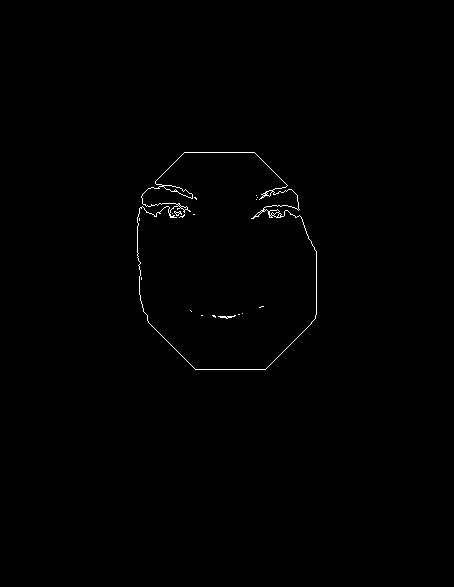
\includegraphics[width=0.53\textwidth]{img/fd3/fail3_faceBorder.png}
  \caption{}
\end{subfigure}%
\begin{subfigure}{.25\textwidth}
  \centering
  
\includegraphics[width=0.53\textwidth]{img/fd3/fail3_eyeCandidates.png}
  \caption{}
\end{subfigure}%
% \begin{subfigure}{.15\textwidth}
%   \centering
%   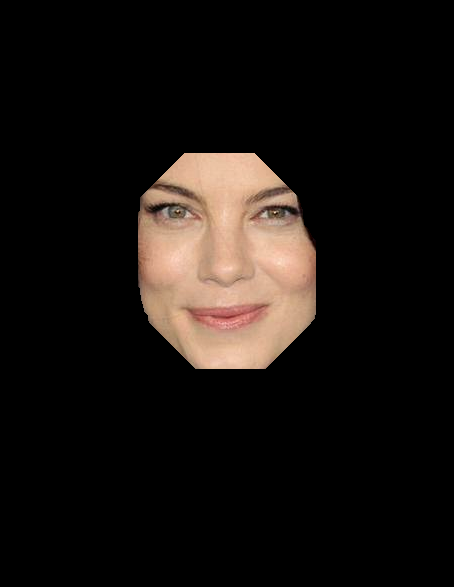
\includegraphics[width=0.53\textwidth]{img/fd3/fail3_faceImage.png}
%   \caption{}
% \end{subfigure}%
% \begin{subfigure}{.15\textwidth}
%   \centering
%   
\includegraphics[width=0.53\textwidth]{img/fd3/fail3_finalEyeMap.png}
%   \caption{}
% \end{subfigure}%
\begin{subfigure}{.25\textwidth}
  \centering
  
\includegraphics[width=0.23\textwidth]{img/fd3/fail3_output.png}
  \caption{}
\end{subfigure}%

\caption{Resonera, Fail3}
\label{fig:fail3}
\end{figure}




\begin{figure}[H]
\centering

\begin{subfigure}{.25\textwidth}
  \centering
  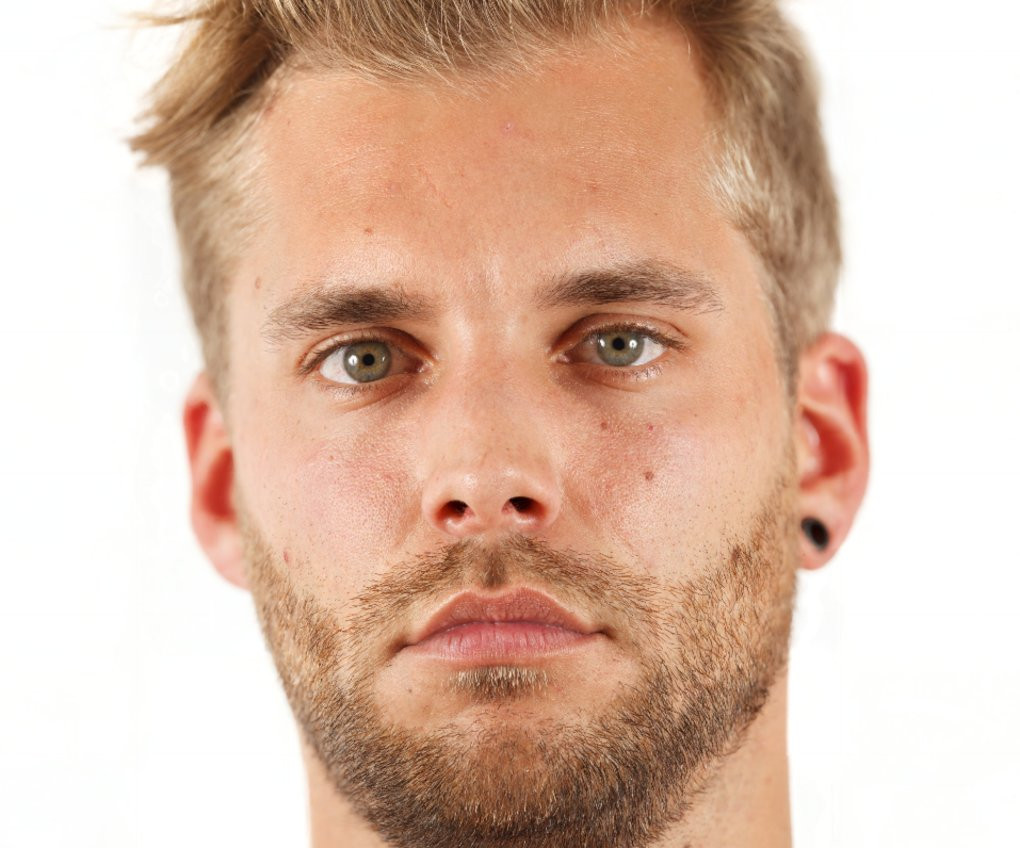
\includegraphics[width=0.95\textwidth]{img/fd3/fail4_input.jpg}
  \caption{}
\end{subfigure}%
\begin{subfigure}{.25\textwidth}
  \centering
  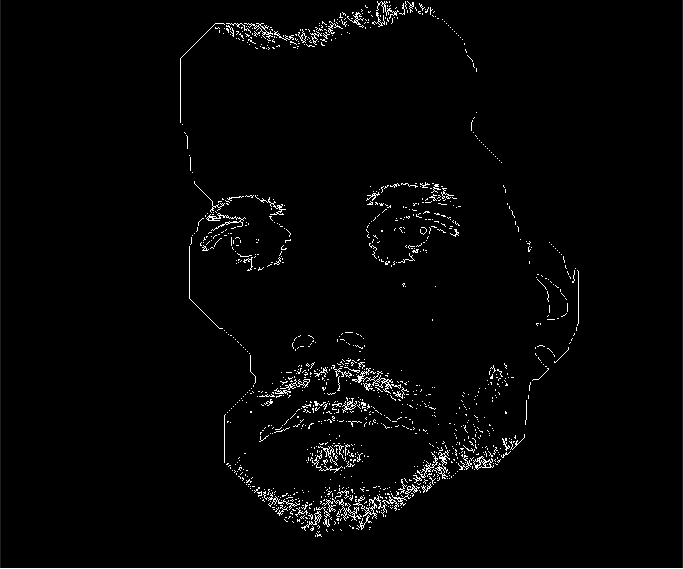
\includegraphics[width=0.95\textwidth]{img/fd3/fail4_faceBorder.png}
  \caption{}
\end{subfigure}%
\begin{subfigure}{.25\textwidth}
  \centering
  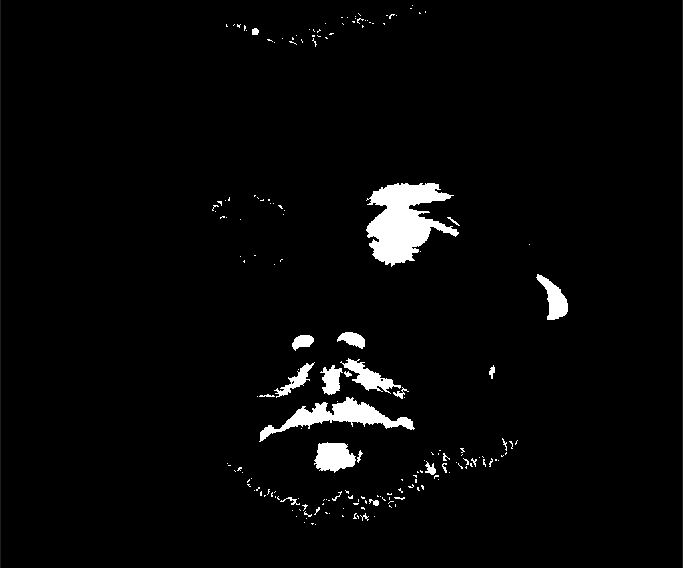
\includegraphics[width=0.95\textwidth]{img/fd3/fail4_eyeCandidates.png}
  \caption{}
\end{subfigure}%
% \begin{subfigure}{.15\textwidth}
%   \centering
%   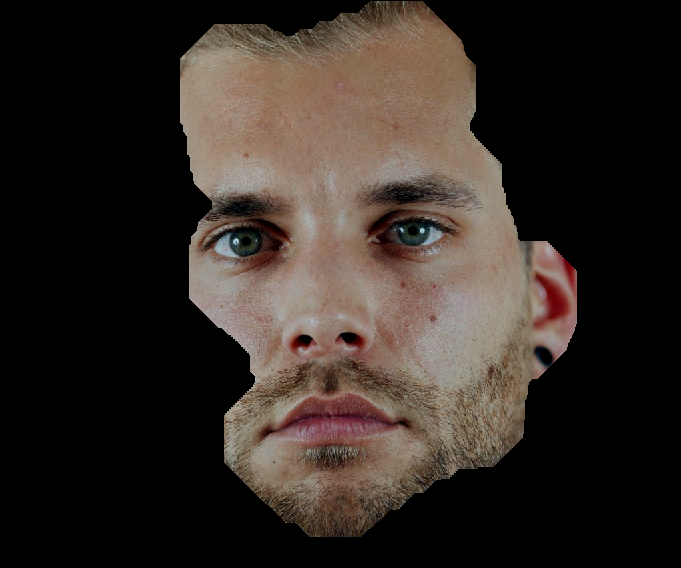
\includegraphics[width=0.95\textwidth]{img/fd3/fail4_faceImage.png}
%   \caption{}
% \end{subfigure}%
% \begin{subfigure}{.15\textwidth}
%   \centering
%   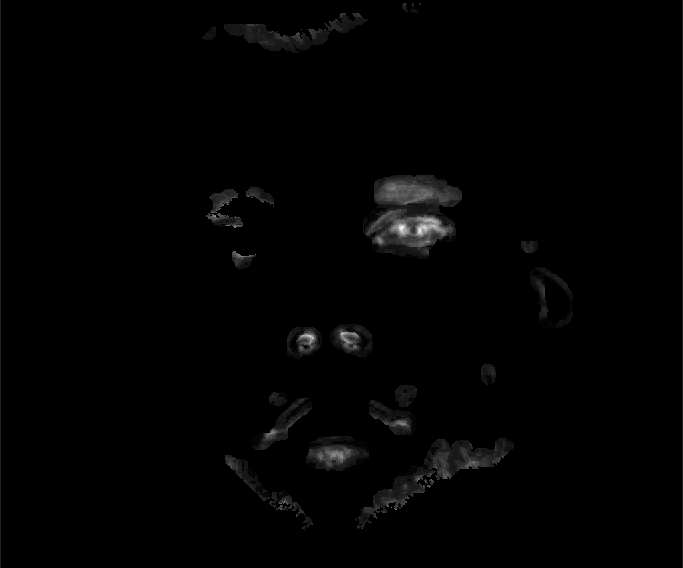
\includegraphics[width=0.95\textwidth]{img/fd3/fail4_finalEyeMap.png}
%   \caption{}
% \end{subfigure}%
\begin{subfigure}{.25\textwidth}
  \centering
  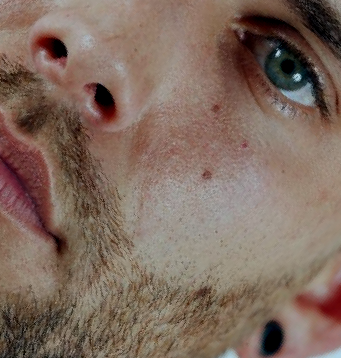
\includegraphics[width=0.53\textwidth]{img/fd3/fail4_output.png}
  \caption{}
\end{subfigure}%

\caption{Resonera, Fail4}
\label{fig:fail4}
\end{figure}







